\documentclass[10pt,letterpaper]{article}
\usepackage[left=.72in,right=1.48in,top=.78in,bottom=.78in,headheight=14pt,marginparwidth=1.22in,marginparsep=.14in]{geometry}
\usepackage{fontspec}
\setmainfont{Liberation Serif}
\setsansfont{Liberation Sans}
\setmonofont[Scale=.75]{DejaVu Sans Mono}
\usepackage{graphicx}
\usepackage{booktabs,longtable,array,tabularx}
\usepackage{amsmath,amssymb,mathtools}
\usepackage{float}
\usepackage{etoolbox}
\AtBeginEnvironment{longtable}{\small}
\usepackage[section]{placeins}
\usepackage{xcolor}
\definecolor{navy}{RGB}{28,50,79}
\definecolor{commentred}{RGB}{158,48,40}
\usepackage{fancyhdr}
\usepackage{fvextra}
\usepackage{microtype}
\usepackage{hyperref}
\hypersetup{colorlinks=true,linkcolor=navy,urlcolor=navy}
\usepackage{caption}
\captionsetup{font=small,labelfont=bf,justification=raggedright,singlelinecheck=false}
\usepackage{enumitem}
\setlist{nosep,topsep=3pt}
\pagestyle{fancy}
\fancyhf{}
\lhead{\small October 20, 2026 Observations from Dr. Claussen}
\rhead{\small Stages 1A--3C}
\cfoot{\thepage}
\setcounter{tocdepth}{2}
\sloppy
\newcommand{\src}[1]{\par\smallskip\noindent\textcolor{navy}{\footnotesize\textbf{Source file(s):} \texttt{#1}}\par}
\newcommand{\takeaway}[1]{\par\smallskip\noindent{\color{commentred}\textbf{Statistical interpretation:} #1}\par\medskip}
\newcommand{\readernote}[1]{%
  \marginpar{\raggedright\scriptsize\color{commentred}%
  \noindent\textbf{READER'S GUIDE}\\[-1pt]
  \rule{\marginparwidth}{1.2pt}\\[3pt]#1}}
\newcommand{\filehint}[1]{\par\smallskip\noindent\textcolor{navy}{\footnotesize\textbf{Find the underlying data:} \texttt{#1}}\par}

\begin{document}
\begin{titlepage}
\vspace*{1.2in}
{\sffamily\Huge\bfseries\color{navy} October 20, 2026\\[4pt]Observations from Dr. Claussen\par}
\vspace{.45in}
{\Large GCV Landscapes, Smoothing Regimes, and Product B Coefficient Sensitivity\par}
\vspace{.2in}
{\large Expanded interpretation of results through Stage 3C\par}
\vspace{.8in}
\noindent\rule{\textwidth}{1pt}
\vspace{.3in}
\noindent\textbf{What is included.} An expanded, source-linked explanation of the completed results, thirteen figures regenerated from the Stage 2 and Stage 3C CSVs, eleven result tables, and red marginal notes providing an accessible explanation of each analytical step. The companion Quarto notebook contains the executable figure- and table-generation code; the four original pasted texts are retained separately in the source package.
\vspace{.25in}
\noindent\textbf{Scope.} This document reports the completed Stages 1A--3C only. It does not assert that Stage 4A refinement, Reiss--Ogden \(h\)-function computation, or a statistical simulation study has been performed. The report ends after Section 11; no code or transcript appendices are embedded.
\vfill
\noindent Prepared as an annotated analytical and discussion record.\\
\textit{Report date requested: October 20, 2026. Compiled from the supplied October 2026 research outputs and four pasted transcripts.}
\end{titlepage}
\tableofcontents
\clearpage
\section{Purpose and source control}
\readernote{This is a guide to already completed analyses. Every displayed finding is linked to a saved result file, not a newly fitted model.}
This note consolidates the completed Stage 1A--3C investigation and the subsequent observations about presentation slides, competing GCV minima, the choice of smoothing parameter, and the estimated Product B coefficient. It intentionally distinguishes (i) reported numerical results read from stage-specific CSV outputs, (ii) interpretation of these results, and (iii) prospective analysis. The appended four transcripts are not silently rewritten; where a transcript reflects an earlier interpretation or a different basis definition, it remains unchanged as requested. Figures and current tables in the main body are linked to exact CSV filenames.

\subsection{How to read this document}
The eleven sections follow the order in which the questions arose. Sections 1--3 establish what was fitted and what was observed. Sections 4--6 compare the graphics from the manual and package-based analyses. Sections 7--8 interpret the two case studies where apparently similar plots lead to different conclusions. Sections 9--10 define the anomaly flags and give a reproducible file lookup. Section 11 sets out the limitations.

The red notes in the right margin are \emph{interpretive annotations}, not additional statistical results. They explain what each display is intended to convey using ordinary language while retaining the statistical distinctions between a sampled local minimum, a criterion-preference comparison and a failed optimizer selection. All calculations reported as results were obtained in the completed Stages 1A--3C.

\subsection{Interpreting the labels on a figure}
Whenever a caption says \emph{manual}, it refers to the independently assembled cubic B-spline basis and integrated curvature penalty. Whenever a caption says \emph{\texttt{mgcv}}, it refers to the package's B-spline model. A plotted \emph{GCV difference} is not the same as the absolute GCV score. The vertical axis, its unit and its reference model must be read before comparing panels. Two curves may have identical shapes after a vertical translation while having very different displayed values.


\noindent\textbf{Reproducibility.} The project directory includes \texttt{October\_20\_2026\_Observations\_from\_Dr\_Claussen.qmd}, \texttt{generate\_figures\_tables.R}, and a \texttt{source\_data/} directory containing the relevant original CSV outputs. The code reads those saved results; it does not re-run model fitting. All figure files have a corresponding source caption below.

\section{What the previous analysis actually studied}
\readernote{We fit one treatment-effect model at each field location. The difficult part is selecting how flexible the Northing adjustment should be.}
At each observed Easting \(e\), the model can be written
\begin{equation}
Y_i(e)=\beta_0(e)+\beta_B(e)I(P_i=B)+f_e(N_i)+\varepsilon_i(e),
\end{equation}
where Product B is the unpenalized effect of interest, and \(f_e\) is a penalized spline adjustment for Northing. Generalized cross-validation is
\begin{equation}
\operatorname{GCV}_e(\lambda)=\frac{24\,\operatorname{RSS}_e(\lambda)}{\{24-\operatorname{EDF}_e(\lambda)\}^{2}}.
\end{equation}
An increase in \(\lambda\) increases the penalty on curvature, typically lowers the smooth's effective degrees of freedom, and often increases residual sum of squares. These effects pull GCV in opposite directions, so the GCV criterion can have multiple stationary points.

\subsection{What the coefficient represents}
The quantity \(\beta_B(e)\) is the adjusted mean Yield difference, Product B minus Product E, at Easting \(e\), conditional on the fitted Northing adjustment. It is an ordinary parametric coefficient within each local fit. The penalty acts on the smooth coefficients rather than directly on \(\beta_B\), but both sets of coefficients are estimated jointly. Consequently, changing \(\lambda\) can still change the reported treatment coefficient when the Product indicator is not orthogonal to the smooth basis after conditioning on the other model columns.

In particular, the estimated trajectory \(e\mapsto\widehat\beta_B(e)\) should not be treated as a direct observation of the true spatial treatment effect. It depends on the chosen smoothing-selection procedure and on the observational structure of the response vectors.


\subsection{The notation \(\log(sp)\) versus \(\log(\lambda)\)}
The original package-fitting code supplies \texttt{sp} as the R argument to \texttt{mgcv::gam()}. In the one-smooth specification used here, \(sp\) plays the role of the package-parameterized smoothing coefficient \(\lambda_{\mathrm{mgcv}}\). Therefore
\begin{equation}
\log(sp)=\log(\lambda_{\mathrm{mgcv}}), \qquad
\lambda_{\mathrm{mgcv}}=\exp\{\log(sp)\}.
\end{equation}
\textbf{But} the numerically constructed manual spline and \texttt{mgcv} use different knot or penalty scaling conventions, so \(\lambda_{\mathrm{manual}}\) and \(\lambda_{\mathrm{mgcv}}\) should not be identified by the same numerical value. All new figures label which parametrization is used.

\paragraph{Worked conversion.} In the one-smooth package model, \(\log(sp)=2.157\) corresponds to \(sp=\exp(2.157)\approx8.64\), not to a GCV value of 2.157. Moving from \(\log(sp)=-3.352\) to \(\log(sp)=2.157\) represents a large multiplicative increase in penalty strength. \texttt{sp} is a variable name; the penalty coefficient in the mathematical criterion is \(\lambda_{\mathrm{mgcv}}\). For this research note all graphical axes use the latter notation.


\subsection{Three different differences that must not be confused}
\begin{align}
\text{Relative GCV profile:}\quad D_e(\lambda)&=\operatorname{GCV}_e(\lambda)-\operatorname{GCV}_{e,\infty},\\
\text{Structural candidate gap:}\quad\Delta_{\mathrm{struct}}(e)&=\operatorname{GCV}_{e,\mathrm{best\ interior}}-\operatorname{GCV}_{e,\infty},\\
\text{Optimizer gap:}\quad\Delta_{\mathrm{opt}}(e)&=\operatorname{GCV}_{e,\mathrm{automatic}}-\operatorname{GCV}_{e,\mathrm{best\ grid}},\\
\text{Coefficient difference:}\quad\Delta_\beta(e)&=\widehat\beta_{B,e,\mathrm{automatic}}-\widehat\beta_{B,e,\mathrm{best\ grid}}.
\end{align}
The subtraction of \(\operatorname{GCV}_{e,\infty}\) does not move any within-Easting stationary point along the horizontal axis because that reference is constant in \(\lambda\). A positive optimizer gap only demonstrates an inferior automatic selection relative to an evaluated candidate, not a proof of the global optimum.

\subsection{A numerical example of why the gaps are different}
At Easting 214, the manual interior candidate has GCV approximately 158.422 and the exact linear limit has GCV approximately 153.498. The \emph{manual structural gap} is therefore about \(+4.924\). Under the separate package implementation the automatic fit has GCV approximately 158.473, while the best tested grid value is about 153.498; the \emph{package optimizer gap} is therefore about \(+4.975\). These quantities are numerically close here, but they compare different pairs of candidates under two different model implementations and must never be used interchangeably.

Similarly, relative GCV is a whole curve, \(D_e(\lambda)\), whereas a structural or optimizer gap is a \emph{single number per Easting}. In the linear-relative heatmap, subtracting \(\mathrm{GCV}_{e,\infty}\) translates one row vertically without altering that row's minima. Its purpose is to make within-Easting improvements directly interpretable.


\section{Stages 1--3C: Summary of completed results}
\readernote{Read these stages in order: check the observations, examine the criterion, then test whether automatic fitting selects a good solution.}
\begin{longtable}{@{}p{1.2cm}p{3.1cm}p{4.2cm}p{5.8cm}@{}}
\caption{Stage summary. Source: \texttt{Stage1B\_Summary.csv; Manual\_Full\_Field\_Summary.csv; Stage3A\_Auto\_vs\_Grid.csv; Stage3B\_Linear\_Screen\_and\_Trajectories.csv; Stage3C\_Auto\_vs\_Grid.csv}.}\label{tab:stage-summary}\\
\toprule
Stage & Experiment & Result & Question answered\\
\midrule
\endfirsthead
\toprule
Stage & Experiment & Result & Question answered\\
\midrule
\endhead
1A & Full-data audit & 4,776 records; 199 Eastings; 24 passes & What is the design?\\
1B & Slice reconciliation & 72 matches & Are original slices unchanged?\\
2 & Manual GCV & 79,600 grid scores; 27 multi-minimum Eastings & What is the manually built GCV landscape?\\
3A & mgcv pilot & 3,600 fixed fits & Can automatic selection miss better grid candidates?\\
3B & Automatic full field & 199 automatic fits; 6 worse than linear & Where does a known lower GCV alternative exist?\\
3C & mgcv full grid & 119,400 fits; 16 inferior selections; 28 multi-minimum Eastings & What is the full evaluated optimizer gap?\\
\bottomrule
\end{longtable}

The complete dataset contains 199 Eastings with a fixed pass-specific design. A three-slice reconciliation matched all observations originally used at Eastings 214, 216 and 218. The manual Stage 2 run evaluated 400 smoothing parameters per Easting, and Stage 3C evaluated 600 package-specific smoothing parameters per Easting. These are \emph{related but not numerically identical} spline constructions.

\subsection{What each completed stage contributed}
\textbf{Stage 1A} checked whether the full harvest file has the expected dimensions, treatment allocations and unique identifiers. Each of the 199 observed Eastings contains 24 harvest passes, including 12 assigned Product B and 12 Product E. The Product, Pair and Northing assignments are fixed within pass. The corresponding source records are \texttt{Easting\_Audit.csv} and \texttt{Pass\_Design\_Audit.csv} from the first audit folder; their conclusions are reflected in the stage summary but their original audit CSVs are not included among the package's figure-generation inputs.

\textbf{Stage 1B} used pass identifiers to reconcile the original three slice exports with the full data. The maximum reported absolute Yield discrepancy was approximately \(3.01\times10^{-12}\) at Easting 214, \(4.01\times10^{-12}\) at Easting 216, and zero at Easting 218. The direct output is \texttt{Stage1B\_Summary.csv}, with record-level matches in \texttt{Stage1B\_Row\_Level\_Reconciliation.csv}. This step establishes correspondence of the inputs, not a statistical conclusion about smoothing.

\textbf{Stage 2} built the cubic B-spline design manually. With ten uncentered spline basis functions, the second-derivative penalty has numerical rank eight, leaving the constant and linear directions unpenalized. The shared model design allows the 24-by-199 Yield matrix to be processed at each of 400 manual grid values. Its principal outputs are the complete \texttt{Manual\_Full\_Field\_Grid.csv} and one-row-per-Easting \texttt{Manual\_Full\_Field\_Summary.csv}.

\textbf{Stage 3A} applied automatic \texttt{mgcv} smoothing and a 600-point fixed grid to six selected Eastings. \textbf{Stage 3B} automatically fitted all 199 Eastings and screened each against the exact linear limit. \textbf{Stage 3C} compared each automatic result with a 600-point \texttt{mgcv} profile over the entire field. The last stage determines the observed 16-Easting optimizer-shortfall set, not a mathematically complete inventory of all possible optima.


\begin{longtable}{@{}p{1.4cm}p{3cm}p{2.8cm}p{3.3cm}p{3.2cm}@{}}
\caption{Original slice manual and mgcv. Source: \texttt{Manual\_Full\_Field\_Summary.csv; Stage3C\_Auto\_vs\_Grid.csv}.}\label{tab:original-slice-manual-and-mgcv}\\
\toprule
Easting & Manual interior GCV & Linear-limit GCV & Automatic mgcv GCV & Best mgcv grid GCV\\
\midrule
\endfirsthead
\toprule
Easting & Manual interior GCV & Linear-limit GCV & Automatic mgcv GCV & Best mgcv grid GCV\\
\midrule
\endhead
214 & 158.422 & 153.498 & 158.473 & 153.498\\
216 & 171.417 & 156.334 & 171.450 & 156.334\\
218 & none detected & 160.229 & 160.229 & 160.229\\
\bottomrule
\end{longtable}

\takeaway{The exact linear-limit scores agree for the two constructions. The finite-smoothing interior scores may differ, even at the same Easting. This is not a contradiction or evidence that the saved results have changed.}

\section{Slides 4 and 14: The two GCV heatmaps}
\readernote{Both heatmaps describe the same idea, but they use different spline constructions. Do not compare their horizontal coordinates as if they were the same units.}
\subsection{Manual GCV, absolute and linear-relative}
\readernote{A color represents a score at one Easting and one smoothing choice. The right panel subtracts the straight-line score from the same row.}
\begin{figure}[H]\centering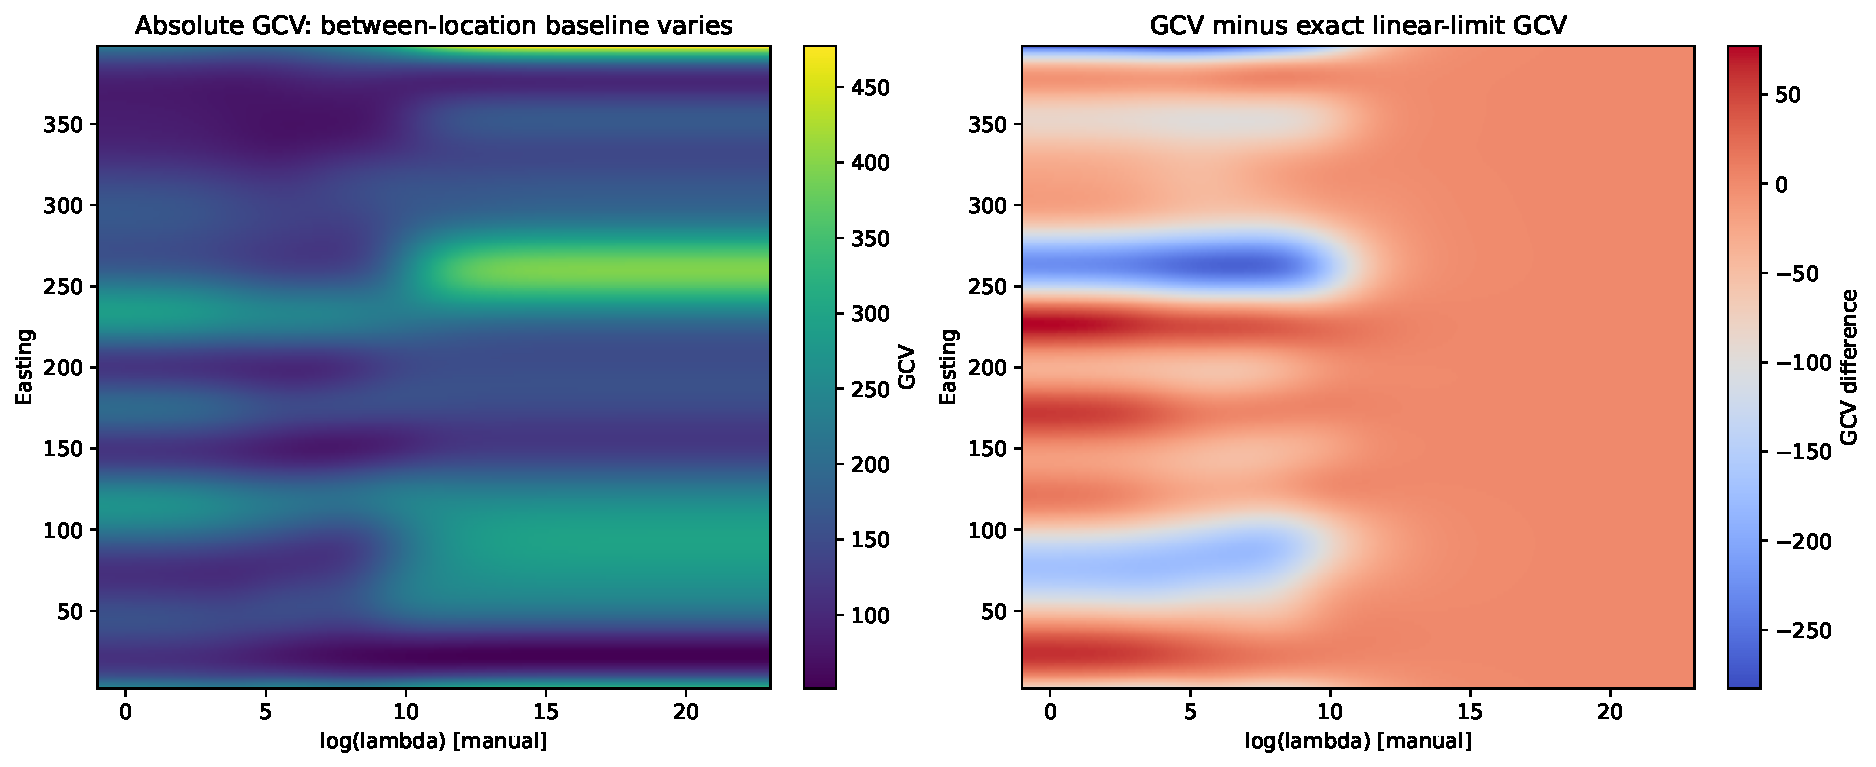
\includegraphics[width=\textwidth]{figures/F01_manual_absolute_relative_heatmaps.pdf}
\caption{The \textbf{manual} absolute GCV heatmap and the manual GCV minus exact linear-limit GCV heatmap. Every row corresponds to one Easting and every column to one value of \(\log(\lambda_{\mathrm{manual}})\). Source: \texttt{Manual\_Full\_Field\_Grid.csv} and \texttt{Manual\_Full\_Field\_Summary.csv}.}\end{figure}
The absolute version shows the criterion's magnitude, which also depends on each Easting's overall residual variation. The relative version isolates how much a particular smoothing parameter improves or worsens the criterion compared with the same Easting's exact linear-limit adjustment.

\paragraph{How to read a heatmap pixel.} Select a particular Easting on the vertical axis, then select a particular \(\ell=\log(\lambda_{\mathrm{manual}})\) on the horizontal axis. The color on the \emph{absolute} panel reports \(\mathrm{GCV}_e(e^\ell)\). The color at the identical location on the \emph{relative} panel reports \(\mathrm{GCV}_e(e^\ell)-\mathrm{GCV}_{e,\infty}\). In other words, the second panel takes the same underlying grid and removes a different constant from each row.

For interpretation, a negative relative score means that the finite-smoothing candidate scores better than the exact linear-limit model for that same Easting, while a positive value means it scores worse. This row-specific centering reduces confounding by differences in criterion levels among Eastings. It does not normalize by Yield variance and it does not make the manual and package penalty scales comparable.

The original presentation's colorbar range was clipped for some extreme relative scores. These regenerated two-panel graphics use explicitly stated color limits and should be examined together with the stored numerical values rather than judging the magnitude of a difference solely from a saturated color.

\takeaway{The relative heatmap is generally more useful for interpreting an interior-versus-linear smoothing preference. The absolute heatmap remains useful for visualizing the overall criterion landscape. Neither heatmap alone establishes that a selected local minimum is globally optimal.}

\subsection{Package-based GCV: a separate horizontal parameter scale}
\readernote{Same conceptual graph, different penalty units. A horizontal shift is not a numerical discrepancy in Yield.}
\begin{figure}[H]\centering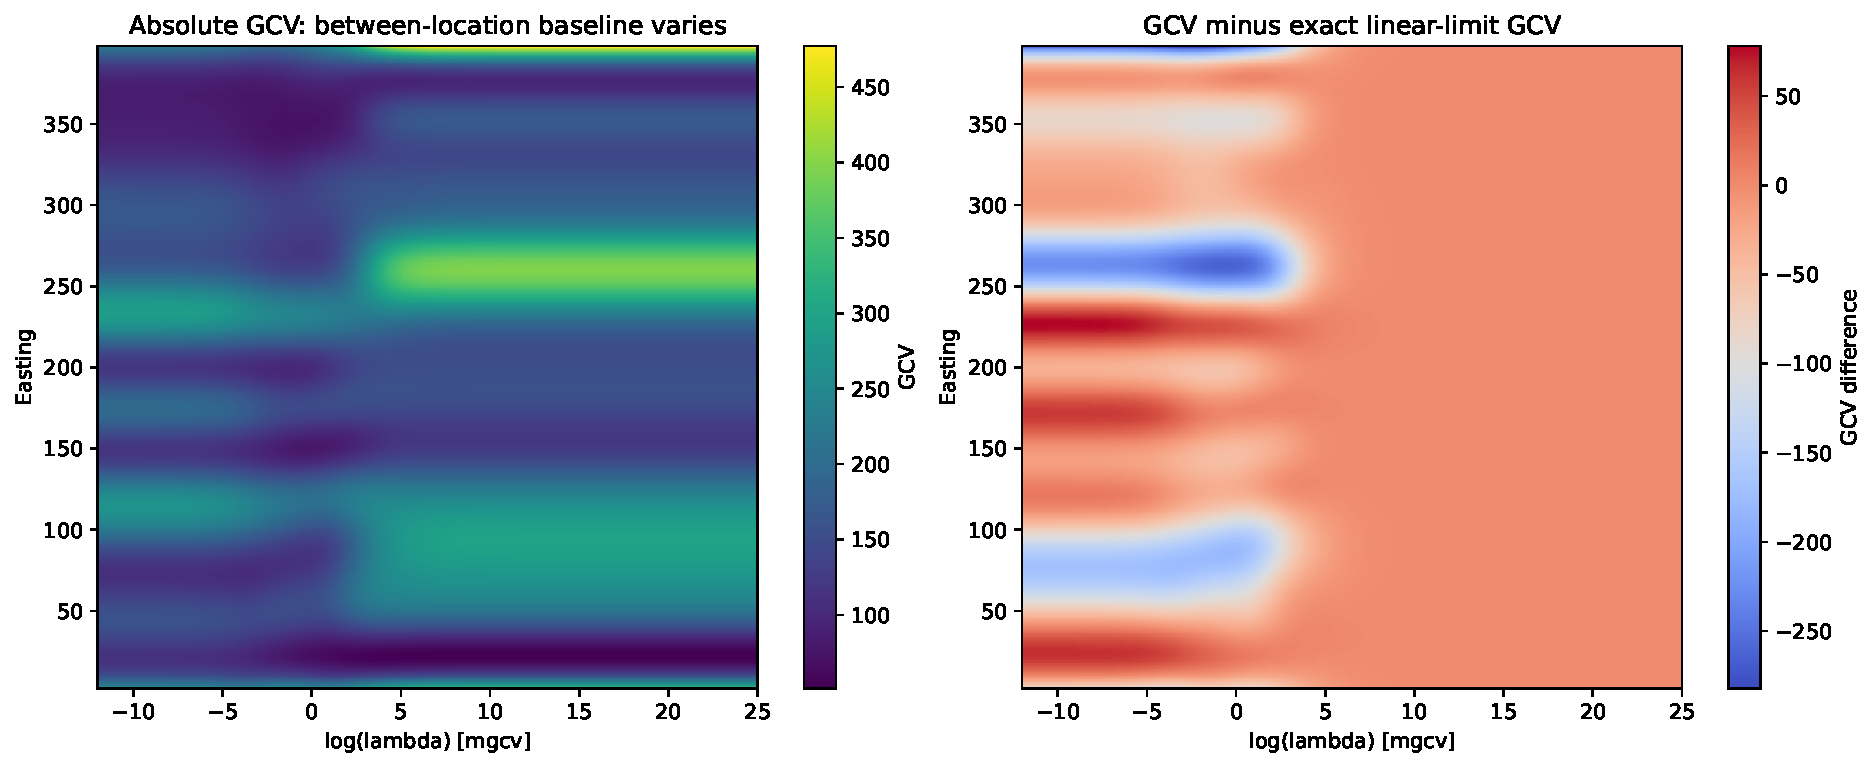
\includegraphics[width=\textwidth]{figures/F02_mgcv_absolute_relative_heatmaps.pdf}
\caption{The \textbf{mgcv} absolute and linear-relative GCV landscapes. Its horizontal axis is \(\log(\lambda_{\mathrm{mgcv}})\), not the manual penalty scale. Source: \texttt{Stage3C\_Full\_Grid.csv} and \texttt{Stage3C\_Auto\_vs\_Grid.csv}.}\end{figure}
\takeaway{Slide 4 and slide 14 should agree about the statistical definition of a GCV profile but should not be expected to have identical horizontal minimum coordinates. They were computed with different penalty constructions.}
\subsection{How to reconcile slides 4, 5, 8, 14 and 17}
Slide 4 displays the manual criterion after row-wise subtraction of the exact linear-limit score. Slide 5 displays the uncentered manual criterion at selected Eastings; a value near 158 on slide 5 can therefore correspond to a difference near +5 on slide 4. Slide 8 compresses an entire manual GCV profile into a single score contrast between the best detected interior candidate and the linear limit. Slide 14 repeats the row-centered landscape for the package-based spline. Slide 17 returns to \emph{absolute} package GCV at individual Eastings. A raw value near 79.7 at Easting 374 can consequently appear near -19.8 on slide 14 because the exact linear-limit GCV is around 99.4.

The equations and source-file labels distinguish these views. A color difference across slides is not interpretable without checking the corresponding subtraction and the package/model identifier. No cross-construction comparison of \(\log\lambda\) should be interpreted as a physical change in smoothness unless basis and penalty scaling have first been aligned.


\section{Slides 5--9: Manual GCV candidates and structural preference}
\readernote{A local dip is a candidate model. Its existence does not imply it has the lowest GCV compared with the nearly linear model.}
\begin{longtable}{@{}p{3.4cm}p{3.4cm}p{3.4cm}@{}}
\caption{Counts of interior minima. Source: \texttt{Manual\_Full\_Field\_Summary.csv; Stage3C\_Auto\_vs\_Grid.csv}.}\label{tab:counts-of-interior-minima}\\
\toprule
Number detected & Manual Eastings & mgcv Eastings\\
\midrule
\endfirsthead
\toprule
Number detected & Manual Eastings & mgcv Eastings\\
\midrule
\endhead
0 & 10 & 10\\
1 & 162 & 161\\
2 & 26 & 27\\
3 & 1 & 1\\
\bottomrule
\end{longtable}

\begin{figure}[H]\centering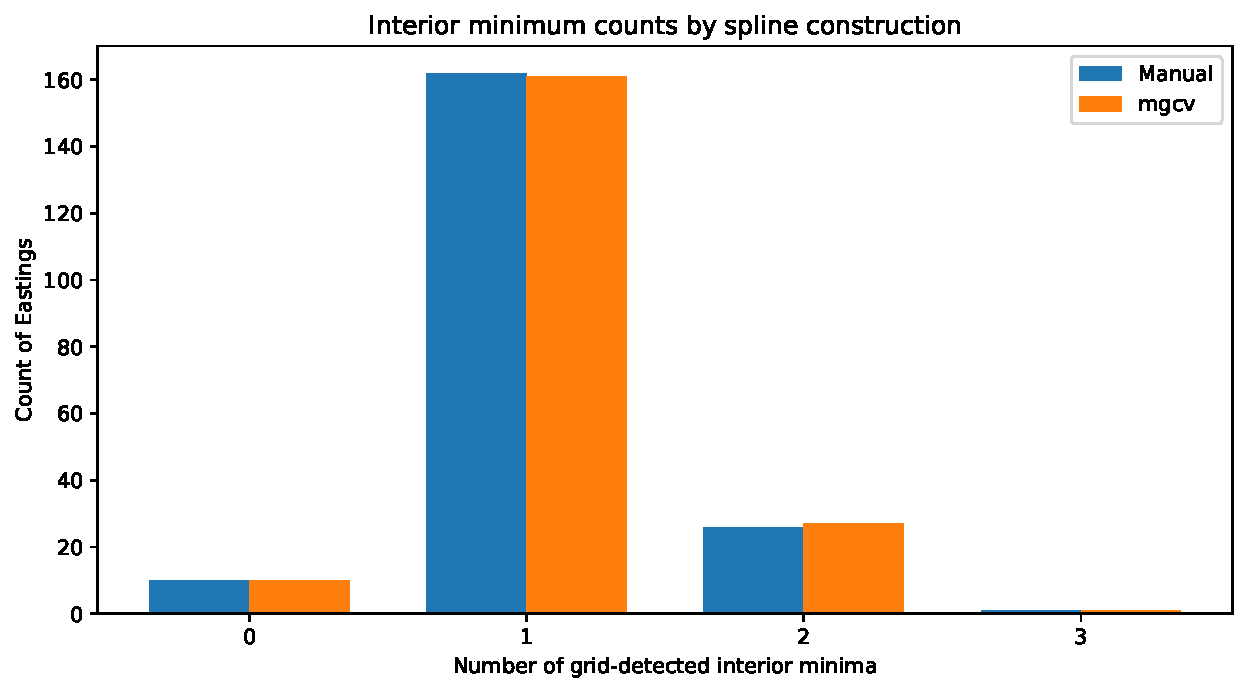
\includegraphics[width=.86\textwidth]{figures/F09_detected_minima_histogram.pdf}
\caption{Distribution of detected interior minima across all 199 Eastings, separately for the manually constructed spline and the \texttt{mgcv} spline. Source: \texttt{Manual\_Full\_Field\_Summary.csv} and \texttt{Stage3C\_Auto\_vs\_Grid.csv}.}\end{figure}
The manual criterion has 27 Eastings with multiple detected interior minima; the package criterion has 28. Easting 80 has two detected package minima but only one detected manual minimum in the saved grid results.

\subsection{What a detected interior minimum means}
\readernote{Two dips mean two nearby favorable choices of smoothness. You still must compare their GCV values.}
On a finite grid \(\ell_1<\ell_2<\cdots<\ell_m\), a candidate minimum is flagged when the GCV score at a grid position is lower than its immediate neighbors, subject to the implementation's admissibility rule. A profile with two detected dips therefore has two different finite smoothing regimes where the numerical curve turns upward on both sides. The flag is about \emph{criterion geometry}; it does not itself say whether either minimum is globally best or whether the automatic optimizer selected the wrong one.

The table and histogram separate the frequencies \(0,1,2,3\) rather than just reporting a total. Manual Stage 2 yields 10, 162, 26 and 1 Eastings in these respective groups; package Stage 3C yields 10, 161, 27 and 1. The difference arises at Easting 80 and should be retained as a model-specific numerical finding, not silently averaged across implementations.


\begin{figure}[H]\centering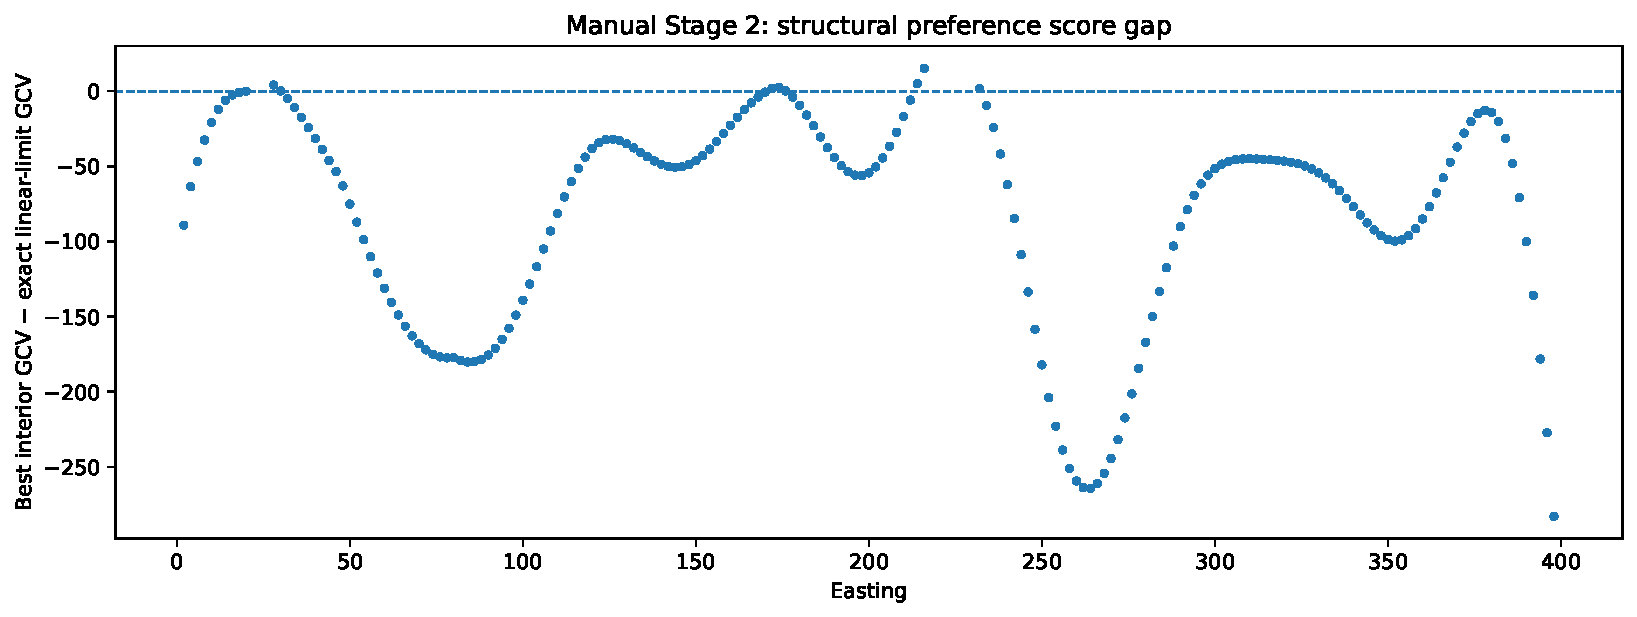
\includegraphics[width=.96\textwidth]{figures/F08_manual_structural_gap.pdf}
\caption{Manual structural gap, best detected interior GCV minus exact linear-limit GCV. Negative values favor a detected interior candidate; positive values favor the linear limit. Undefined where no qualifying interior candidate exists. Source: \texttt{Manual\_Full\_Field\_Summary.csv}.}\end{figure}
\begin{figure}[H]\centering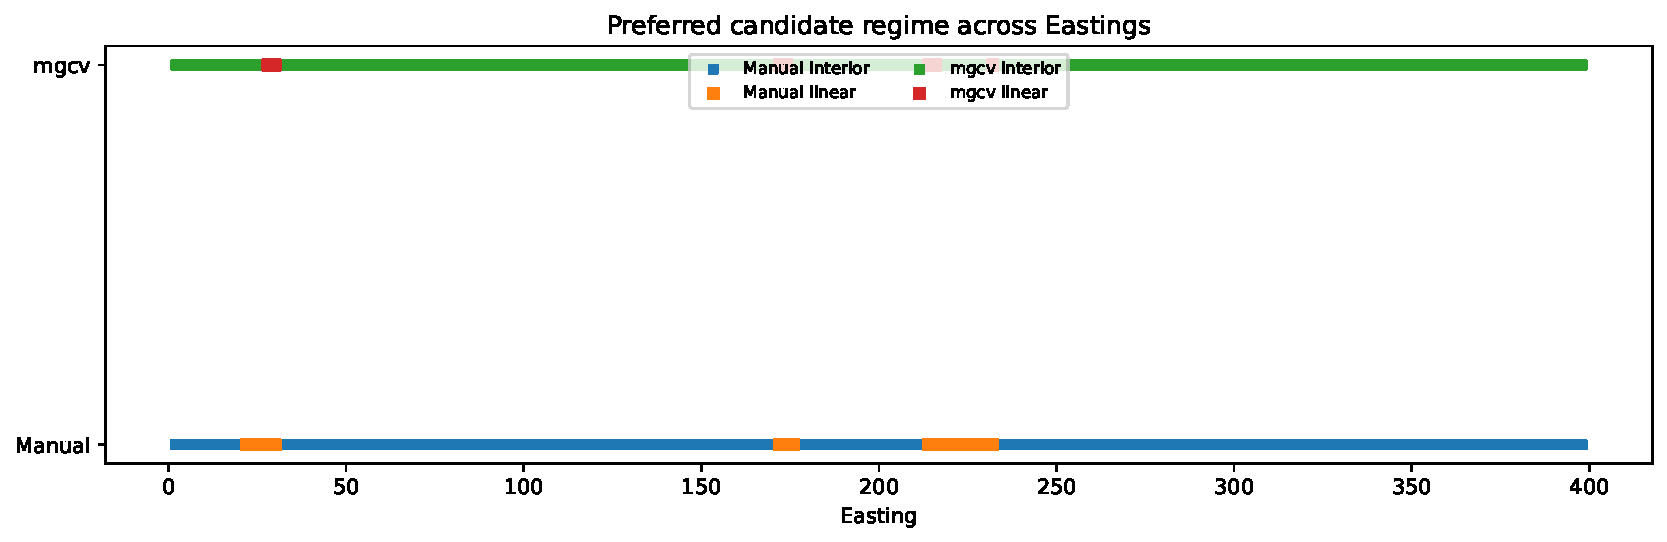
\includegraphics[width=.98\textwidth]{figures/F10_regime_preference_map.pdf}
\caption{Preferred detected candidate by Easting for the manual and package criteria. The change in classification near Easting 176 illustrates basis-dependent near-ties, not a plotting transcription error. Source: \texttt{Manual\_Full\_Field\_Summary.csv} and \texttt{Stage3C\_Auto\_vs\_Grid.csv}.}\end{figure}
\takeaway{The manual slides primarily diagnose structural criterion preference. The automatic package slides separately test what numerical solution the optimizer actually returned. These are not interchangeable questions.}
\subsection{Six observed preference boundaries are not six proved spatial discontinuities}
The manual Stage 2 candidate classifications change between 20--22, 30--32, 170--172, 176--178, 212--214 and 232--234. The package grid yields broadly corresponding boundaries but shifts the 176--178 boundary to 174--176. These are pairs of measured Eastings with different candidate labels. They say which evaluated regime had the lower criterion score \emph{at the sampled slices}; they do not prove a discontinuity in the underlying agricultural response or a zero crossing at a precisely located continuous Easting.


\section{Slides 10--17: What automatic fitting found}
\readernote{We now compare what the software selected with other smoothing parameters we explicitly evaluated.}
\begin{longtable}{@{}p{1.8cm}p{2.8cm}p{3.2cm}p{2.0cm}p{2.5cm}@{}}
\caption{Six Easting pilot comparison. Source: \texttt{Stage3A\_Auto\_vs\_Grid.csv}.}\label{tab:six-easting-pilot-comparison}\\
\toprule
Easting & Auto GCV & Best grid GCV & Gap & Product B gap\\
\midrule
\endfirsthead
\toprule
Easting & Auto GCV & Best grid GCV & Gap & Product B gap\\
\midrule
\endhead
212 & 145.664 & 145.666 & -0.002 & +0.003\\
214 & 158.473 & 153.498 & +4.975 & -0.358\\
216 & 171.450 & 156.334 & +15.116 & -0.418\\
218 & 160.229 & 160.229 & -0.000 & -0.000\\
232 & 223.937 & 223.937 & -0.000 & -0.000\\
234 & 228.609 & 228.610 & -0.000 & -0.002\\
\bottomrule
\end{longtable}

\begin{figure}[H]\centering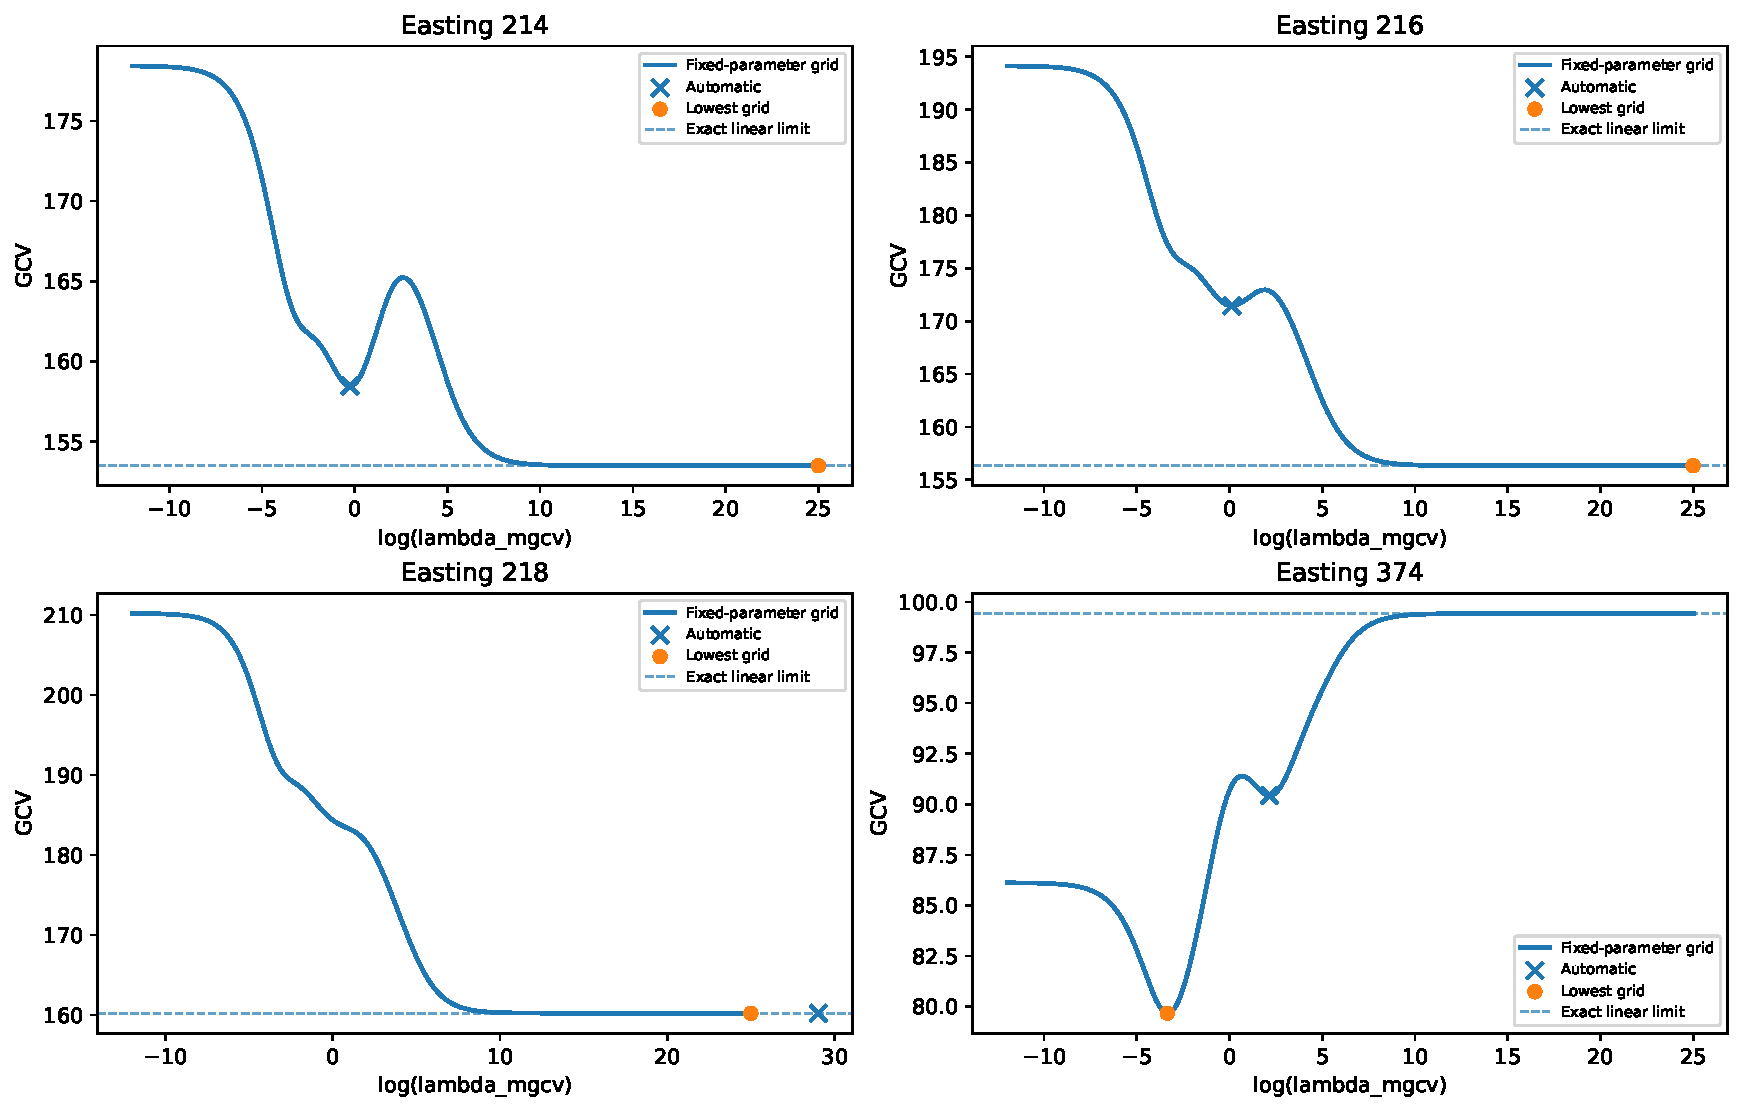
\includegraphics[width=.95\textwidth]{figures/F03_four_mgcv_GCV_profiles.pdf}
\caption{Full fixed-grid GCV curves at Eastings 214, 216, 218, and 374. The automatic selection (cross), lowest grid candidate (filled circle), and exact linear-limit score (dashed line) are shown within each panel's own GCV scale. Source: \texttt{Stage3C\_Full\_Grid.csv} and \texttt{Stage3C\_Auto\_vs\_Grid.csv}.}\end{figure}
\begin{figure}[H]\centering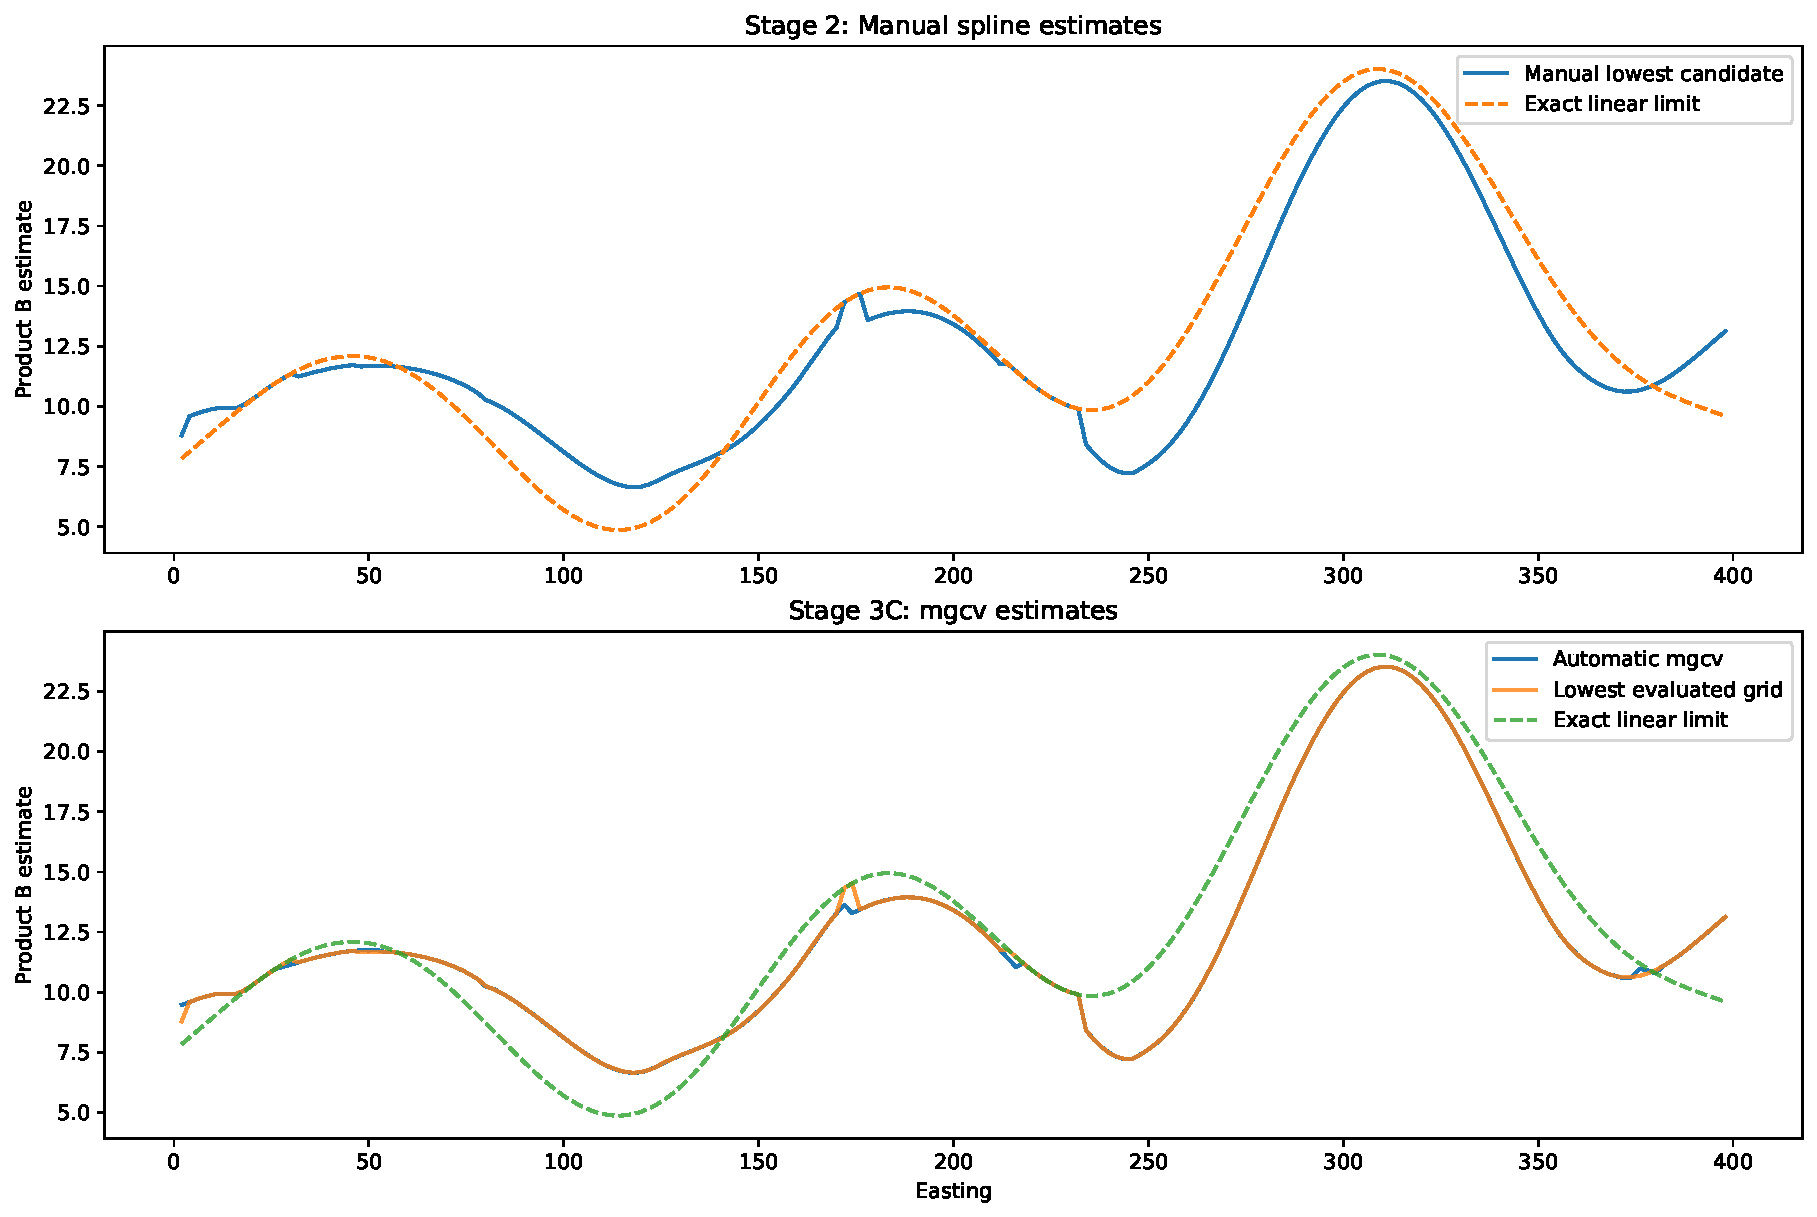
\includegraphics[width=.96\textwidth]{figures/F06_product_coefficient_trajectories.pdf}
\caption{Estimated Product B trajectories across Eastings. The top panel belongs to the manual construction; the bottom panel to automatic and fixed-grid \texttt{mgcv}. The two finite-smoothing constructions can produce different coefficients even though their exact linear limits agree. Source: \texttt{Manual\_Full\_Field\_Summary.csv} and \texttt{Stage3C\_Auto\_vs\_Grid.csv}.}\end{figure}
\begin{figure}[H]\centering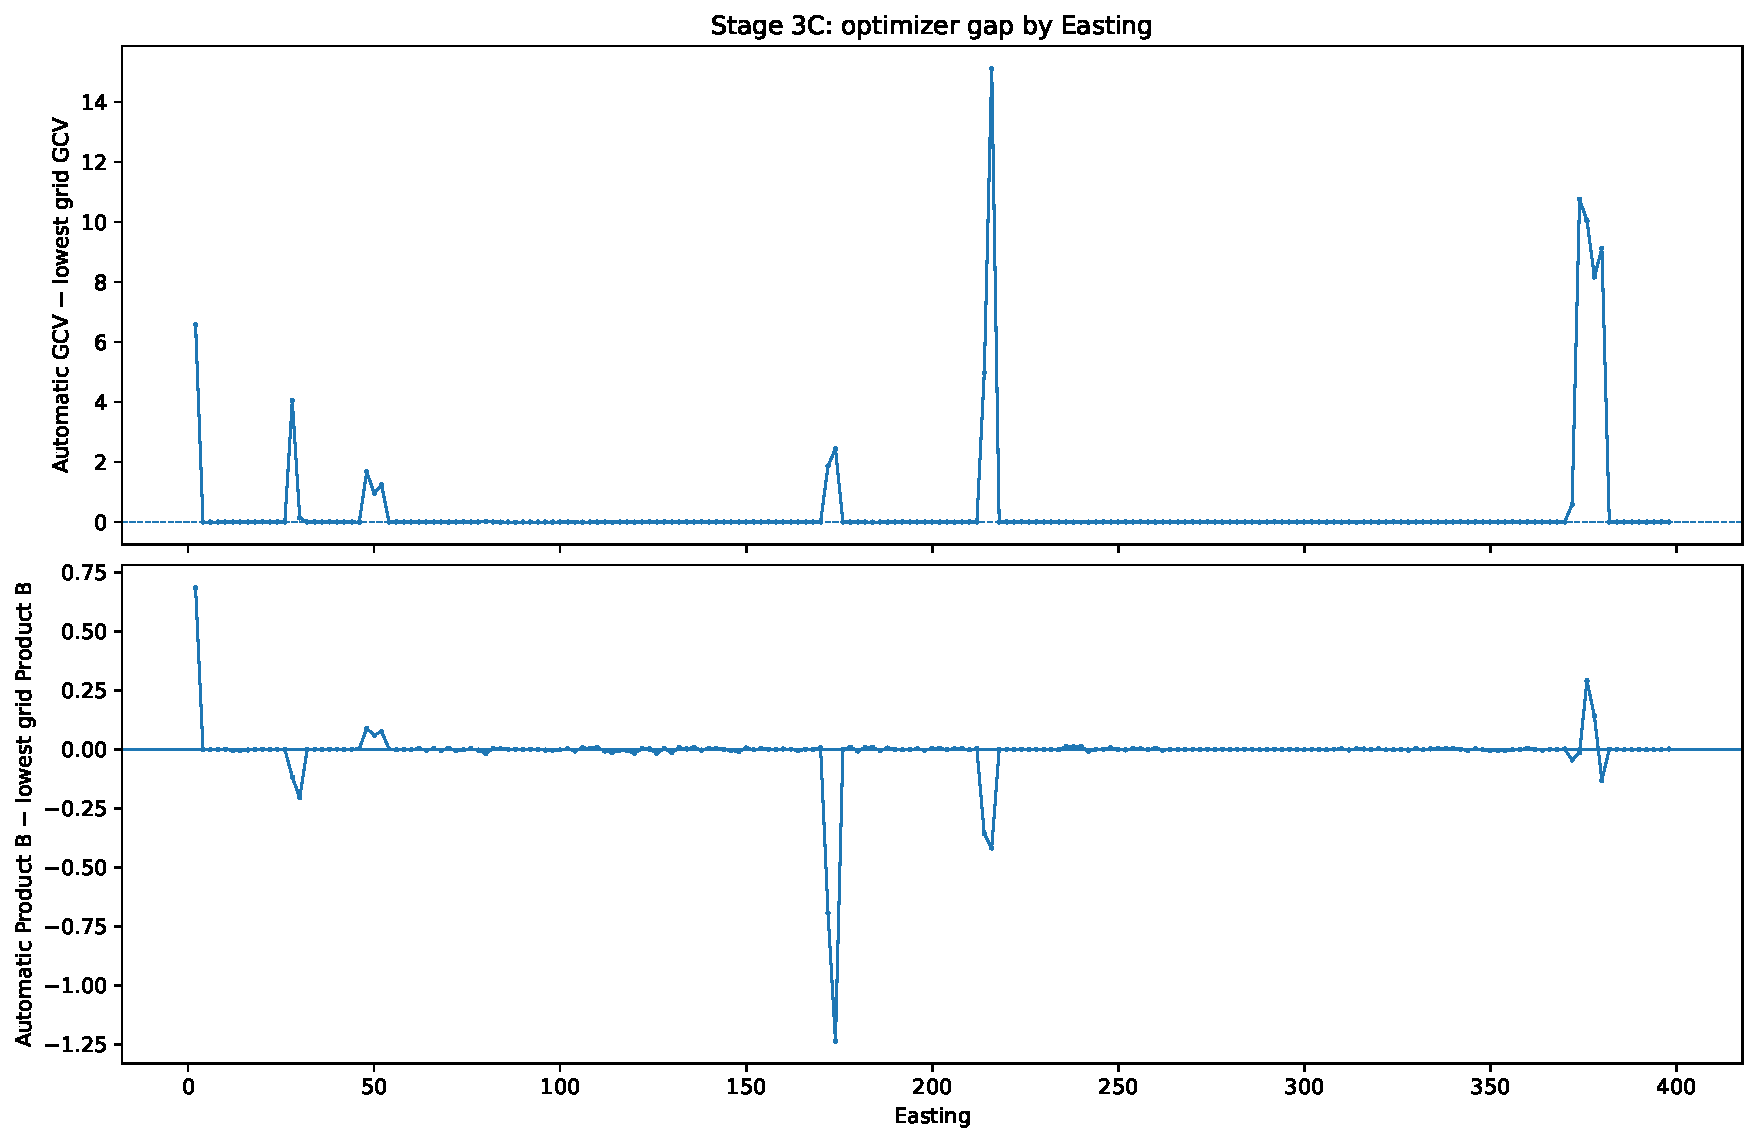
\includegraphics[width=.92\textwidth]{figures/F07_optimizer_gaps_vs_coefficient_sensitivity.pdf}
\caption{Automatic-minus-lowest-grid GCV and Product B differences over the full field. The objective-score gap and its impact on the scientific coefficient need not have similar magnitudes. Source: \texttt{Stage3C\_Auto\_vs\_Grid.csv}.}\end{figure}
\begin{longtable}{@{}p{1.8cm}p{2.6cm}p{3.8cm}p{2.7cm}@{}}
\caption{Sixteen inferior automatic selections. Source: \texttt{Stage3C\_Auto\_vs\_Grid.csv}.}\label{tab:sixteen-inferior-automatic-selections}\\
\toprule
Easting & GCV gap & Coefficient difference & Interior minima\\
\midrule
\endfirsthead
\toprule
Easting & GCV gap & Coefficient difference & Interior minima\\
\midrule
\endhead
2 & 6.581 & +0.686 & 2\\
28 & 4.049 & -0.117 & 1\\
30 & 0.135 & -0.205 & 1\\
48 & 1.675 & +0.089 & 3\\
50 & 0.961 & +0.060 & 2\\
52 & 1.244 & +0.076 & 2\\
80 & 0.017 & -0.017 & 2\\
172 & 1.868 & -0.694 & 1\\
174 & 2.439 & -1.237 & 1\\
214 & 4.975 & -0.358 & 1\\
216 & 15.116 & -0.418 & 1\\
372 & 0.587 & -0.045 & 2\\
374 & 10.761 & -0.014 & 2\\
376 & 10.050 & +0.291 & 2\\
378 & 8.169 & +0.141 & 2\\
380 & 9.132 & -0.131 & 2\\
\bottomrule
\end{longtable}

\begin{figure}[H]\centering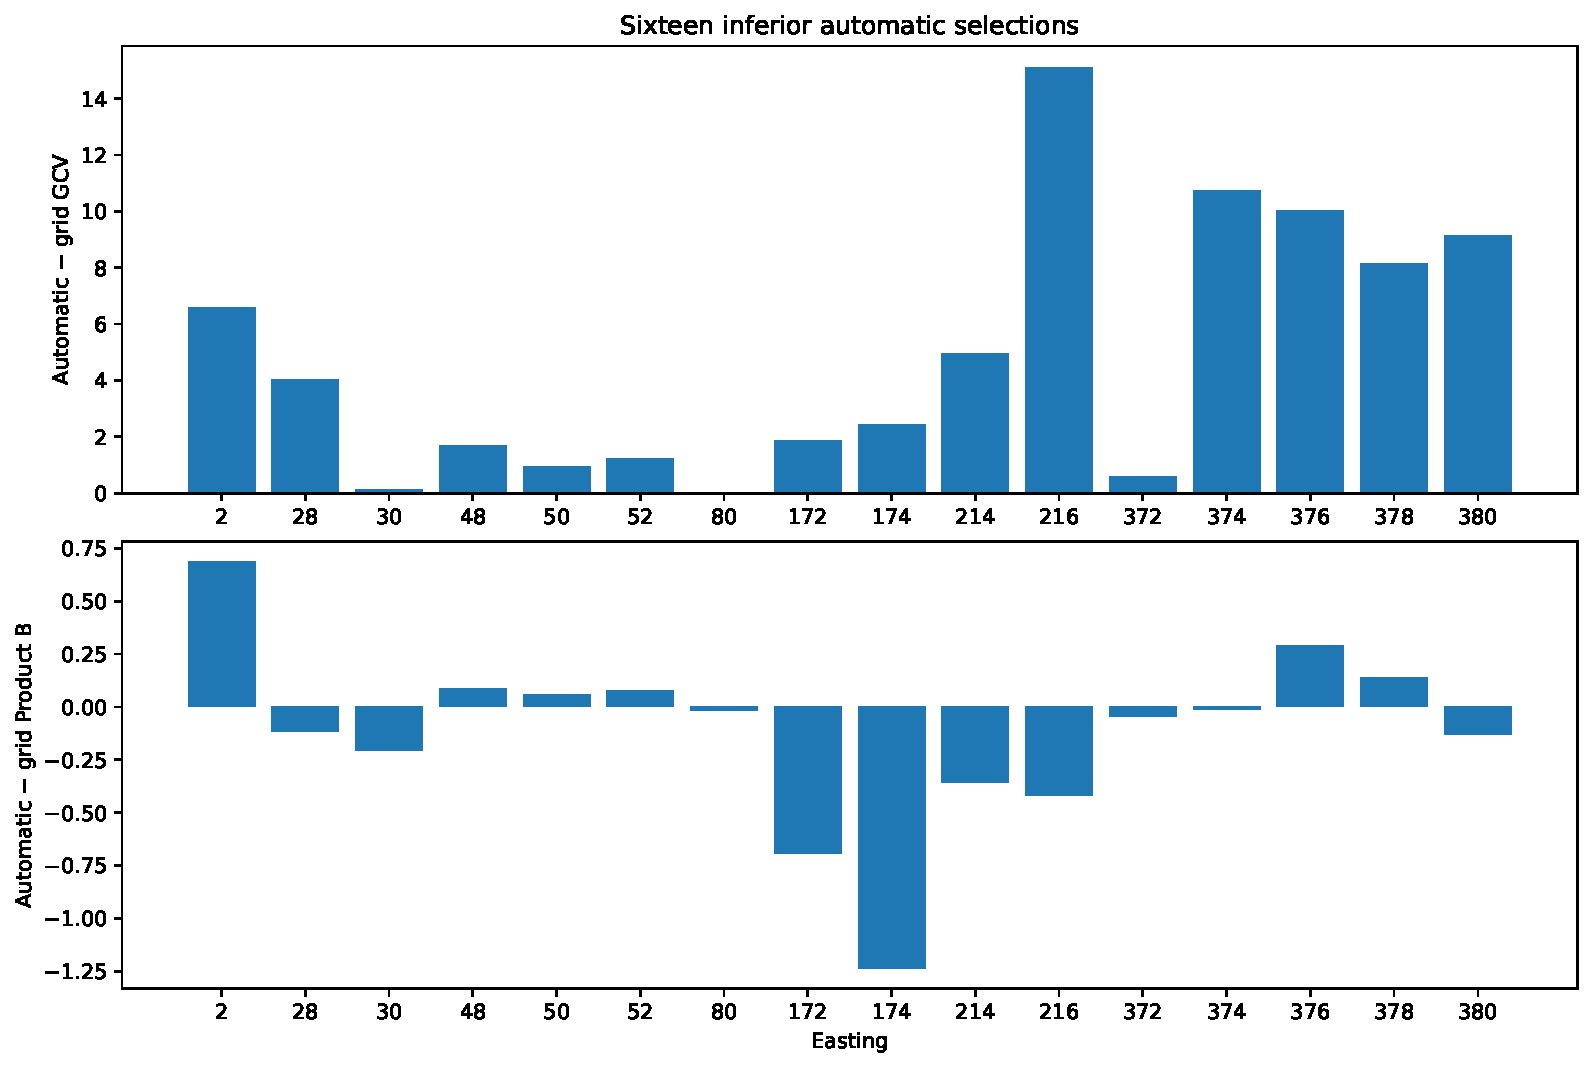
\includegraphics[width=.92\textwidth]{figures/F11_sixteen_inferior_automatic_selections.pdf}
\caption{The 16 Eastings whose automatic GCV scores exceed at least one evaluated fixed-grid alternative beyond the prespecified numerical tolerance. Source: \texttt{Stage3C\_Auto\_vs\_Grid.csv}.}\end{figure}
\takeaway{At 16 Eastings, a tested fixed smoothing parameter gave a lower GCV score than the automatic return value. Six of these already failed a linear-limit comparison; ten needed other finite smoothing candidates to reveal the issue.}

\subsection{Why the 16-Easting list matters more than a simple convergence report}
\readernote{A fit can converge without being the lowest-scoring tested fit. Convergence and optimality are not synonyms.}
Convergence is an algorithmic stopping condition. It indicates that an optimizer has satisfied its numerical termination criterion, not that the returned location has the lowest score over every smoothing parameter that could have been tried. At Eastings 214 and 216, the high-penalty, nearly linear alternative has a lower GCV score than the automatic solution. At Eastings 374--380, the better candidate is often a \emph{more flexible finite-penalty} solution instead. These are different kinds of optimizer shortfall.

The 16 locations are 2, 28, 30, 48, 50, 52, 80, 172, 174, 214, 216, 372, 374, 376, 378 and 380. The accompanying score differences identify the criterion shortfall; the Product B differences show whether that shortfall matters for the scientific parameter. Neither a large score gap nor multiple minima alone is a sufficient indicator of a large treatment-coefficient discrepancy.


\section{Easting 176: A near-tie that affects the Product coefficient}
\readernote{A very small difference in model-selection scores can change the chosen smoothing regime and substantially change the treatment estimate.}
\begin{longtable}{@{}p{2.2cm}p{3cm}p{3cm}p{4.9cm}@{}}
\caption{Easting 176 comparison. Source: \texttt{Manual\_Full\_Field\_Summary.csv; Stage3C\_Auto\_vs\_Grid.csv}.}\label{tab:easting-176-comparison}\\
\toprule
Model & Interior GCV & Linear GCV & Preferred treatment coefficient\\
\midrule
\endfirsthead
\toprule
Model & Interior GCV & Linear GCV & Preferred treatment coefficient\\
\midrule
\endhead
Manual & 146.3298 & 146.2541 & 14.6881\\
mgcv & 146.2077 & 146.2541 & 13.4384\\
\bottomrule
\end{longtable}

\begin{figure}[H]\centering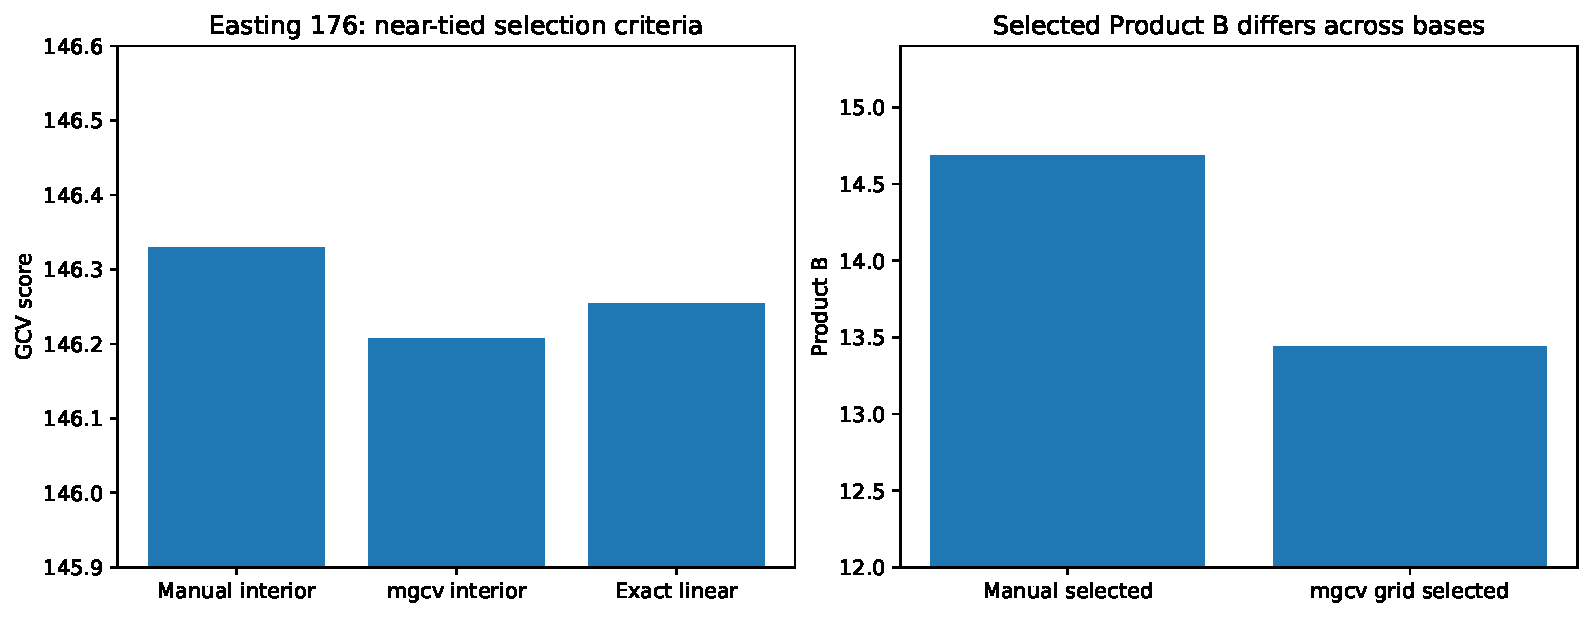
\includegraphics[width=.91\textwidth]{figures/F12_easting_176_basis_sensitivity.pdf}
\caption{Easting 176. The manual and package-based interior criteria lie close to the exact linear-limit score; the favored regime nevertheless differs between constructions. Source: \texttt{Manual\_Full\_Field\_Summary.csv} and \texttt{Stage3C\_Auto\_vs\_Grid.csv}.}\end{figure}
The manual comparison favors the linear limit by roughly 0.076 GCV units, while the package fixed-grid comparison favors an interior solution by approximately 0.046 GCV units. This difference in preferred regime corresponds to about 1.25 units in the reported Product B estimate. This should be treated as \emph{basis-sensitive numerical selection}, not as evidence that one estimate is closer to the unknown treatment effect.

\subsection{Why the two coefficients can be far apart}
\readernote{A small difference in predictive score can select a different smooth and change the adjusted treatment effect.}
At Easting 176, the manual candidate ordering favors the linear limit by roughly 0.076 GCV units, whereas the package grid favors an interior candidate by roughly 0.046. A change of this small magnitude in the criterion comparison changes the chosen smoothing regime. The linear adjustment and a flexible Northing curve partial out different components of Yield variation; because Product B is estimated after this adjustment, the estimated Product B contrast can move markedly. The displayed difference of approximately 1.25 is therefore a \emph{difference between reported model-specific estimates}, not a direct measure of bias or measurement error.

This near-tie also clarifies the apparent mismatch between the manual and package regime-transition maps: the manual transition is reported at 176--178, while the package transition occurs at 174--176. The observed Eastings are discrete; neither pair of labels proves the presence or precise location of a continuous crossing between samples.


\section{Easting 374: Why GCV rises as smoothing increases}
\readernote{The curve moves left-to-right over smoothing choices AT Easting 374, not from one Easting to another. Greater smoothing does not guarantee lower GCV.}
At Easting 374 the package grid shows two interior local minima. The automatic parameter lies near the higher-scoring local minimum.

\paragraph{Read the horizontal axis carefully.} A single point in the plot is a model fitted using the \emph{same 24 Yield observations at Easting 374} but with a different smoothing parameter. Left-to-right movement changes \(\lambda_{\mathrm{mgcv}}\), not geographic position. Because \(\ell=\log\lambda_{\mathrm{mgcv}}\), a displacement of one unit on the horizontal axis multiplies the penalty by \(e\approx2.718\). The axis is logarithmic so a very wide range of positive penalty strengths can be inspected in one plot.

\paragraph{What the two valleys say.}
\readernote{At the same Easting, the flexible minimum beats the smoother automatic fit. Its lower score does not guarantee a truer treatment coefficient.} The first sampled minimum occurs near \(\ell=-3.352\) (\(\lambda\approx0.035\)), has GCV approximately 79.671 and a smooth EDF near 7.911. The automatic result is near \(\ell=2.157\) (\(\lambda\approx8.64\)), with GCV approximately 90.432 and smooth EDF near 3.081. The automatic solution is thus more heavily penalized, less flexible and inferior by approximately 10.761 GCV units to the best evaluated grid candidate. This is a \emph{within-profile comparison}, not a comparison of two Eastings.
 \emph{The GCV increase is along the within-Easting log-smoothing axis, not an increase in GCV from Easting 216 to 374.}
\begin{longtable}{@{}p{3.3cm}p{3.2cm}p{2cm}p{2.7cm}p{2.2cm}@{}}
\caption{Easting 374 stationary candidates. Source: \texttt{Stage3C\_Interior\_Grid\_Dips.csv; Stage3C\_Auto\_vs\_Grid.csv}.}\label{tab:easting-374-stationary-candidates}\\
\toprule
Candidate & log(lambda mgcv) & GCV & Smooth EDF & Product B\\
\midrule
\endfirsthead
\toprule
Candidate & log(lambda mgcv) & GCV & Smooth EDF & Product B\\
\midrule
\endhead
Grid interior 1 & -3.3523 & 79.6709 & 7.9112 & 10.6287\\
Grid interior 2 & 2.1452 & 90.4318 & 3.0899 & 10.6108\\
Automatic & 2.1569 & 90.4316 & 3.0814 & 10.6145\\
\bottomrule
\end{longtable}

\begin{longtable}{@{}p{4.2cm}p{4cm}p{2.6cm}p{2.8cm}@{}}
\caption{Easting 374 criterion along grid. Source: \texttt{Stage3C\_Full\_Grid.csv; Stage3C\_Interior\_Grid\_Dips.csv}.}\label{tab:easting-374-criterion-along-grid}\\
\toprule
Position & log(lambda mgcv) & GCV & Smooth EDF\\
\midrule
\endfirsthead
\toprule
Position & log(lambda mgcv) & GCV & Smooth EDF\\
\midrule
\endhead
Grid left edge & -12.000 & 86.120 & 9.000\\
First interior dip & -3.352 & 79.671 & 7.911\\
Second interior dip & 2.145 & 90.432 & 3.090\\
Grid right edge & 25.000 & 99.434 & 1.000\\
\bottomrule
\end{longtable}

\begin{figure}[H]\centering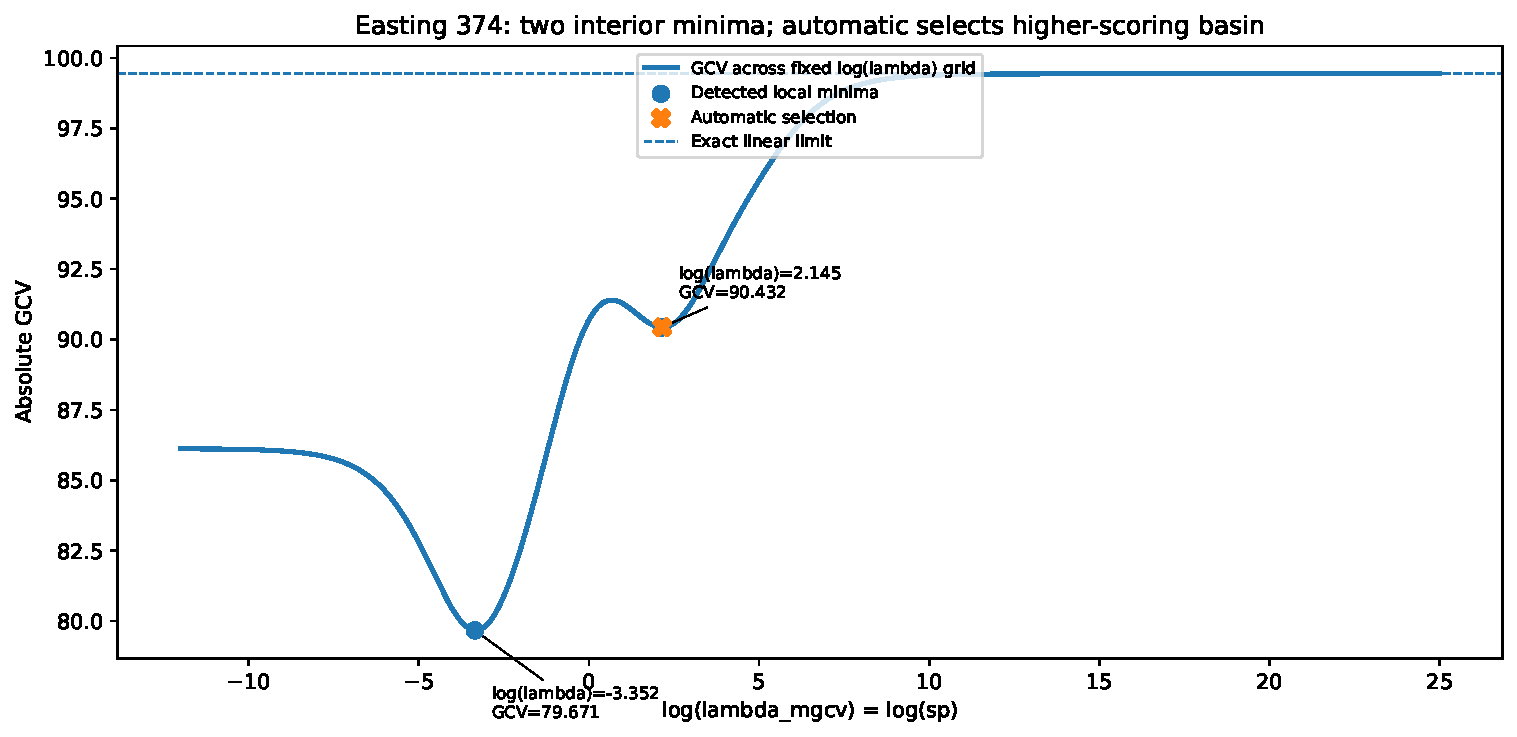
\includegraphics[width=.96\textwidth]{figures/F04_Easting_374_two_minima.pdf}
\caption{Easting 374 fixed-parameter GCV profile. One interior minimum has GCV near 79.671, while the automatic parameter lies near another minimum with GCV near 90.432; the exact linear-limit score is about 99.434. Source: \texttt{Stage3C\_Full\_Grid.csv}, \texttt{Stage3C\_Interior\_Grid\_Dips.csv}, and \texttt{Stage3C\_Auto\_vs\_Grid.csv}.}\end{figure}
\begin{figure}[H]\centering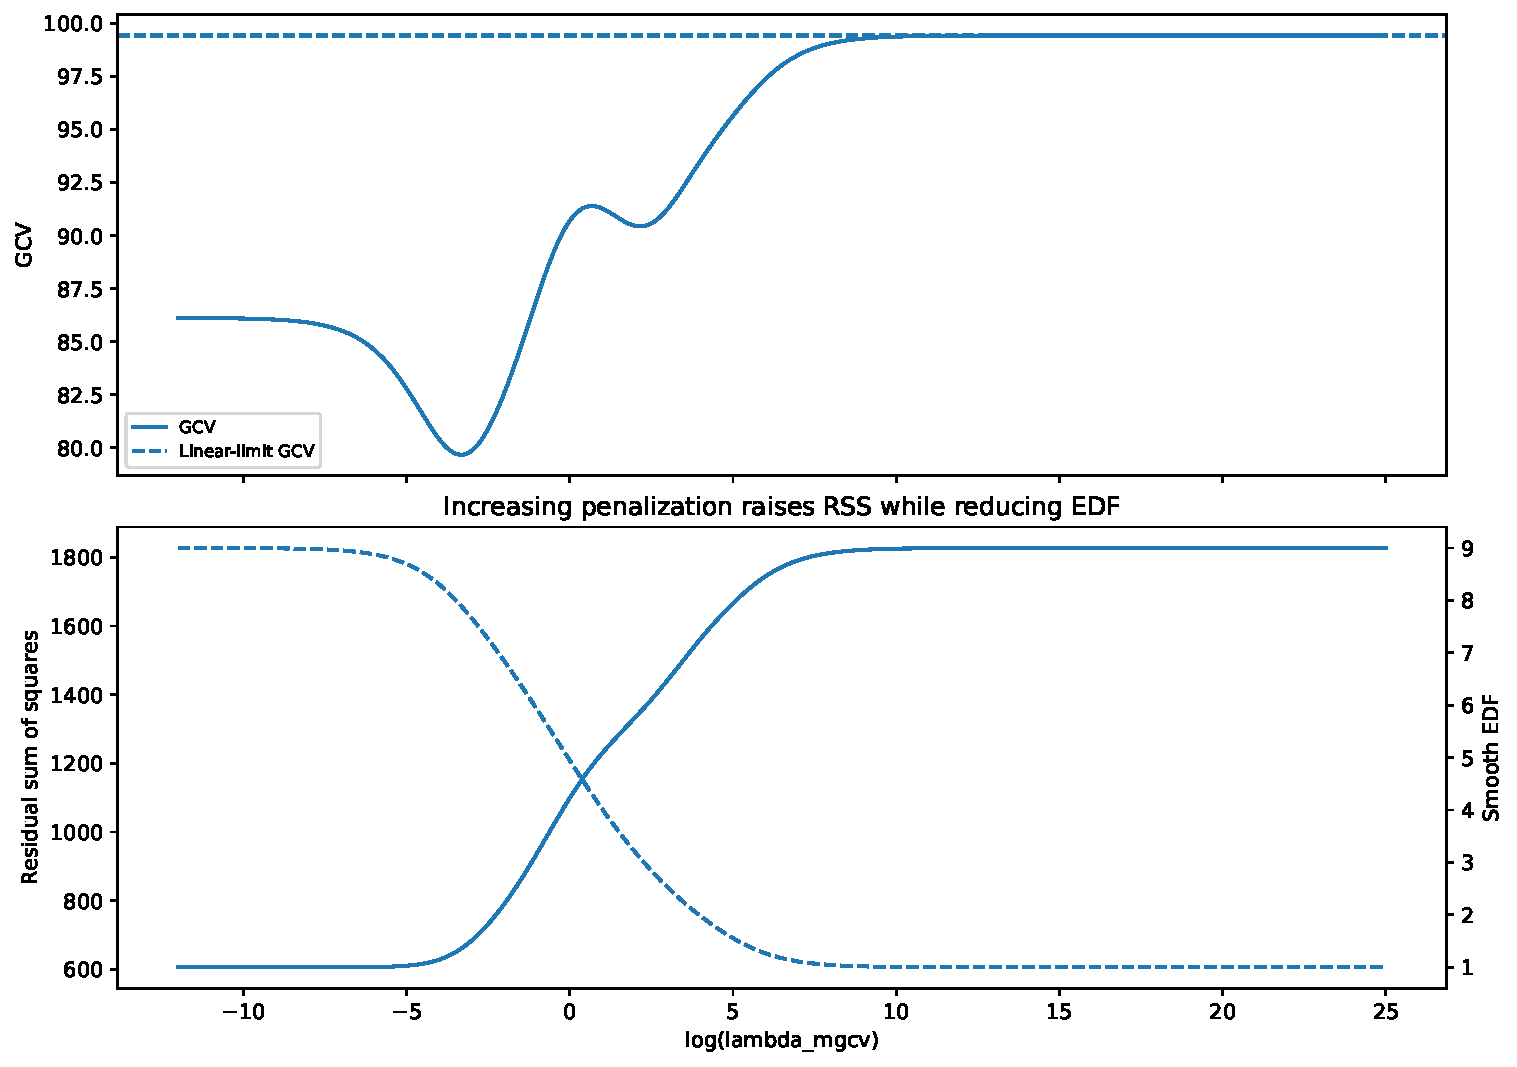
\includegraphics[width=.92\textwidth]{figures/F05_Easting_374_GCV_RSS_EDF.pdf}
\caption{Easting 374: GCV and the opposing fit-versus-complexity effects. With increasing smoothing, the residual sum of squares increases while smooth EDF decreases. In the strongly penalized regime here, fit deterioration outweighs the complexity reduction and GCV rises. Source: \texttt{Stage3C\_Full\_Grid.csv} and \texttt{Stage3C\_Auto\_vs\_Grid.csv}.}\end{figure}
The two competing effects follow immediately from
\begin{equation}
\operatorname{GCV}(\lambda)=\frac{24\operatorname{RSS}(\lambda)}{\left\{24-\operatorname{EDF}(\lambda)\right\}^2}.
\end{equation}
Increasing \(\lambda\) typically lowers EDF (favors parsimony) and increases RSS (worsens fit). Their net impact on the ratio depends on the response. GCV is therefore not a monotone function of the smoothing parameter.

\subsection{Why a GCV curve can bend upward, downward and upward again}
The fit and complexity terms should be considered separately. A finite increase in \(\lambda\) weakens the curvature component of the fit and reduces the effective degrees of freedom. In the denominator of GCV this generally increases \(24-\mathrm{EDF}\), which tends to lower the criterion if the residual sum of squares were unchanged. Meanwhile the residual sum of squares can increase because the fit can no longer follow the observations as closely. The numerator then tends to raise GCV. Nothing requires the two effects to balance in only one place.

This is not a contradiction between the heatmap and the individual profile. The heatmap shows a whole \emph{family} of curves at different Eastings. Each horizontal row is a separate criterion function and may have a different number or placement of stationary points.
 In our package specification \(sp=\lambda_{\mathrm{mgcv}}\), so the original slide's ``log(sp)'' is simply \(\log(\lambda_{\mathrm{mgcv}})\), not a special alternative statistical criterion.

\paragraph{The numerator and denominator move in opposite directions.} The two valleys can be understood by separating the components of generalized cross-validation. At the first minimum the reported residual sum of squares is approximately 658.92 with total EDF about 9.911; near the automatic minimum RSS is about 1348.61 with total EDF about 5.081; and the exact linear limit has RSS about 1827.09 with total EDF 3. In the GCV ratio, reductions in EDF reward lower complexity, but the observed RSS rises enough to make the more strongly penalized model score worse. These are descriptive, not causal, comparisons of fitted models.

\begin{longtable}{@{}p{1.7cm}p{2.2cm}p{3.2cm}p{7.1cm}@{}}
\caption{Selected coefficient sensitivity contrasts. Source: \texttt{Stage3C\_Auto\_vs\_Grid.csv}.}\label{tab:selected-coefficient-sensitivity-contrasts}\\
\toprule
Easting & GCV gap & Product B difference & Interpretation\\
\midrule
\endfirsthead
\toprule
Easting & GCV gap & Product B difference & Interpretation\\
\midrule
\endhead
174 & +2.439 & -1.237 & Larger coefficient sensitivity\\
374 & +10.761 & -0.014 & Small coefficient sensitivity despite larger GCV gap\\
\bottomrule
\end{longtable}

\takeaway{At 374, the optimizer is substantially inferior in GCV but the Product B effect changes little. At 174, the coefficient difference is much larger despite a smaller score gap. Criterion performance and coefficient sensitivity need separate diagnostics.}

\section{Full multiple-minimum anomaly taxonomy}
\readernote{A location can have several simultaneous flags. Counting minima, measuring optimizer gaps, and measuring treatment-effect changes are different diagnostics.}
\begin{longtable}{@{}p{2.2cm}p{6.2cm}p{6.4cm}@{}}
\caption{Anomaly taxonomy. Source: \texttt{GCV\_Stage3C\_Anomaly\_Taxonomy\_All\_Eastings.csv; Stage3C\_Auto\_vs\_Grid.csv}.}\label{tab:anomaly-taxonomy}\\
\toprule
Code & Rule & Meaning\\
\midrule
\endfirsthead
\toprule
Code & Rule & Meaning\\
\midrule
\endhead
M0--M3 & 0, 1, 2, or 3 interior minima & Number of detected candidate minima\\
A & At least 2 interior minima & Multiple-minimum profile\\
B & Automatic minus grid GCV > 0.0001 & Inferior automatic solution\\
C & Automatic minus linear GCV > 0.0001 & Inferior to linear alternative\\
D & Best interior GCV minus linear GCV > 0.0001 & Linear preferred\\
E & Best interior GCV minus linear GCV < -0.0001 & Interior preferred\\
F & Absolute Product B difference >= 0.25 & Provisional coefficient-sensitivity flag\\
G & Minima GCV spread >= 5 & Provisional widely-spaced score flag\\
H & Grid best at right edge & Strongly penalized candidate\\
\bottomrule
\end{longtable}

\begin{figure}[H]\centering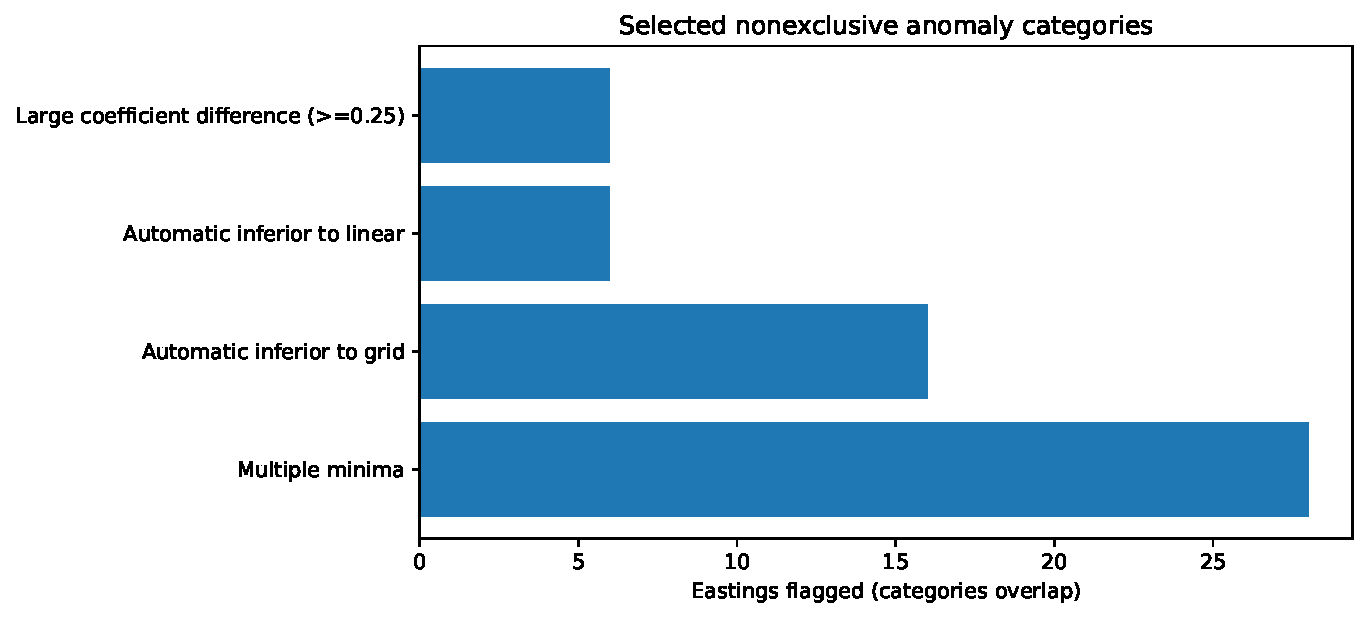
\includegraphics[width=.93\textwidth]{figures/F13_taxonomy_counts.pdf}
\caption{Selected overlapping anomaly categories, including multiple interior minima, inferior automatic solutions, and large coefficient changes. These are descriptive flags, not hypothesis tests. Source: \texttt{GCV\_Stage3C\_Anomaly\_Taxonomy\_All\_Eastings.csv} and \texttt{Stage3C\_Auto\_vs\_Grid.csv}.}\end{figure}
\begin{longtable}{@{}p{1.8cm}p{3cm}p{4.2cm}p{2.5cm}@{}}
\caption{Twenty eight multiple minimum Eastings. Source: \texttt{Stage3C\_Auto\_vs\_Grid.csv; Stage3C\_Interior\_Grid\_Dips.csv}.}\label{tab:twenty-eight-multiple-minimum-eastings}\\
\toprule
Easting & Interior minima & Auto worse than grid? & GCV gap\\
\midrule
\endfirsthead
\toprule
Easting & Interior minima & Auto worse than grid? & GCV gap\\
\midrule
\endhead
2 & 2 & Yes & 6.581\\
4 & 2 & No & -0.004\\
6 & 2 & No & -0.002\\
8 & 2 & No & -0.001\\
44 & 2 & No & -0.001\\
46 & 2 & No & -0.004\\
48 & 3 & Yes & 1.675\\
50 & 2 & Yes & 0.961\\
52 & 2 & Yes & 1.244\\
80 & 2 & Yes & 0.017\\
122 & 2 & No & -0.000\\
124 & 2 & No & -0.000\\
126 & 2 & No & -0.002\\
128 & 2 & No & -0.000\\
130 & 2 & No & -0.002\\
132 & 2 & No & -0.000\\
182 & 2 & No & -0.002\\
184 & 2 & No & -0.003\\
186 & 2 & No & -0.001\\
188 & 2 & No & -0.001\\
190 & 2 & No & -0.000\\
372 & 2 & Yes & 0.587\\
374 & 2 & Yes & 10.761\\
376 & 2 & Yes & 10.050\\
378 & 2 & Yes & 8.169\\
380 & 2 & Yes & 9.132\\
382 & 2 & No & -0.001\\
384 & 2 & No & -0.000\\
\bottomrule
\end{longtable}


\subsection{How to apply the labels without losing information}
\readernote{Use overlapping flags; one Easting can have several kinds of anomalies at once.}
Every Easting receives one of \(M0,M1,M2,M3\), reporting the number of detected interior minima. The additional flags can overlap. Flag \(A\) identifies a multi-minimum profile; \(B\) identifies an automatic result with GCV more than \(10^{-4}\) above the lowest evaluated grid score; \(C\) identifies an automatic result inferior to the exact linear limit; and \(D,E\) contrast the best detected interior candidate with the exact linear limit. Flags \(F\) and \(G\) are exploratory severity conventions (coefficient difference at least 0.25; candidate score spread at least five), not thresholds derived from a probability model. Flag \(H\) means the minimum among grid points is at the right boundary; it is not proof of the exact infinite-penalty optimum.

Easting 374 illustrates the \(A+B\) combination: it has two interior minima and a demonstrably inferior automatic selection, yet a very small Product B discrepancy. Easting 174 illustrates the need for nonexclusive labels: only one qualifying interior minimum is detected, but a different candidate has a better score and a considerably different Product B estimate. Accordingly, a taxonomy limited to \(A\) would miss some of the most consequential coefficient differences.

\takeaway{A useful classification is multilabel: criterion geometry, optimizer performance, and coefficient consequence are distinct dimensions. Restricting attention to multiple-minimum locations alone would overlook meaningful cases such as 174, 214, and 216.}

\section{Where to recover every plotted number}
\readernote{Every exhibit traces back to a specific CSV. Filter by Easting first, then examine grid positions or candidate rows.}
\begin{longtable}{@{}p{3.2cm}p{10.7cm}@{}}
\caption{Primary saved output files. The filenames refer to the \texttt{source\_data/} copies included with this document and to the identically named originals in the user's stage directories.}\\
\toprule Analysis & Direct saved input\\\midrule\endfirsthead
\toprule Analysis & Direct saved input\\\midrule\endhead
Manual GCV scores & \texttt{Manual\_Full\_Field\_Grid.csv}, filter by \texttt{Easting}, 400 observations per location.\\
Manual preference & \texttt{Manual\_Full\_Field\_Summary.csv}, one row per Easting.\\
Manual minima & \texttt{Manual\_Candidate\_Minima.csv}, candidate-level records.\\
Six-Easting pilot & \texttt{Stage3A\_Auto\_vs\_Grid.csv}.\\
Automatic/linear trajectory & \texttt{Stage3B\_Linear\_Screen\_and\_Trajectories.csv}.\\
Full package GCV scores & \texttt{Stage3C\_Full\_Grid.csv}, filter \texttt{Easting = 374} to find 600 points.\\
Package stationary candidates & \texttt{Stage3C\_Interior\_Grid\_Dips.csv}, filter by Easting.\\
Optimizer and coefficient gaps & \texttt{Stage3C\_Auto\_vs\_Grid.csv}, one row per Easting.\\
Taxonomy flags & \texttt{GCV\_Stage3C\_Anomaly\_Taxonomy\_All\_Eastings.csv}.\\
\bottomrule\end{longtable}
\subsection{Practical Excel and R lookup procedure}
The principal summary \texttt{Stage3C\_Auto\_vs\_Grid.csv} has one row per Easting. In Excel, apply \emph{Data $\rightarrow$ Filter} to the \texttt{Easting} field and enter 374; the columns \texttt{Automatic\_GCV}, \texttt{Best\_Grid\_GCV}, \texttt{Automatic\_LogLambda} and \texttt{Auto\_Minus\_Best\_Grid\_Beta} provide the summary comparison. To recover the actual curve, open \texttt{Stage3C\_Full\_Grid.csv}, filter \texttt{Easting = 374}, and sort the 600 rows by \texttt{LogLambda}. To recover the two interior candidates, filter \texttt{Stage3C\_Interior\_Grid\_Dips.csv} to the same Easting.

The folder-name prefix distinguishes the experiment: \texttt{02\_Manual\_Full\_Field} contains the manual construction, while \texttt{03C\_MGCV\_Fixed\_Grid\_Full\_Field} contains the package-based calculation. A CSV file displayed with an Excel icon is still plain comma-separated text. The source package supplied with this document mirrors the relevant inputs under \texttt{source\_data/}; it does not require another run of \texttt{mgcv} merely to render the figures.

\section{Limits of the findings and work still to do}
\readernote{These are numerical comparisons against tested alternatives, not proofs of global optimality or proof of the true treatment effect.}
The observed minima are currently discrete-grid candidates; Stage 4A refinement and Stage 5's Reiss--Ogden stationary-point analysis remain planned.
A better evaluated alternative demonstrates an optimizer shortfall relative to that candidate, not mathematical global optimality. Similarly, a changed estimate of Product B does not establish which estimate is closer to the unknown true effect.

\subsection{Why numerical evidence is not the same as formal inference}
The current analyses demonstrate lower-scoring \emph{evaluated} alternatives. They do not establish that every mathematical stationary point has been enumerated or that the smallest evaluated score is the global minimum on \((0,\infty)\). Refining a candidate inside its neighboring grid interval is the purpose of Stage 4A. Checking the reparameterized residual-maker structure and the theoretical crossings \(h_2(\lambda)=h_3(\lambda)\) is the objective of Stage 5, and these calculations have not been executed in the completed results.

Further, neighboring response vectors share the same harvest passes, and the original Yield series may have been smoothed along Easting before the pointwise analysis. Accordingly, the estimated coefficient trajectory does not represent 199 statistically independent trials. The completed analysis measures criterion and coefficient \emph{sensitivity}; it does not supply confidence intervals or sampling-theoretic error rates for anomaly detection.

\subsection{What a prospective study would need}
A controlled simulation could hold the true Product coefficient fixed or vary it according to a known smooth function while varying the design overlap, error correlation and spline specification. Only with known truth could we determine whether a criterion-regime switch increases bias, variance or mean squared error and whether a proposed anomaly flag has useful false-positive properties. These are directions for future research, not completed experiments included in the tables above.


\end{document}
